\section{Capacity study: results}
\label{sec:results}

\subsection{Shared structure collapses Hebbian recall}

Figure~\ref{fig:recall} shows exact recall against load for prototype patterns at 10\% noise, Fig.~\ref{fig:capacity} the capacity $P_{50}$ against overlap, and Table~\ref{tab:capacity} the values at 10\% noise. For independent balanced patterns ($\rho = 0$), Hebbian $P_{50}$ is \N{c:proto:0.0:hebb:10} [\N{c:proto:0.0:hebb:10:lo}, \N{c:proto:0.0:hebb:10:hi}]. It falls to \N{c:proto:0.1:hebb:10} at $\rho = 0.1$, \N{c:proto:0.2:hebb:10} at 0.2, \N{c:proto:0.3:hebb:10} at 0.3, and \N{c:proto:0.4:hebb:10} at 0.4. From $\rho = 0.5$, the crossing lies between 2 and 3 patterns, and recall at three patterns is \N{r:proto:0.5:hebb:10:3} at $\rho = 0.5$, \N{r:proto:0.6:hebb:10:3} at 0.6 to 0.8, and \N{r:proto:0.9:hebb:10:3} at 0.9.

\begin{figure}[t]
\centering
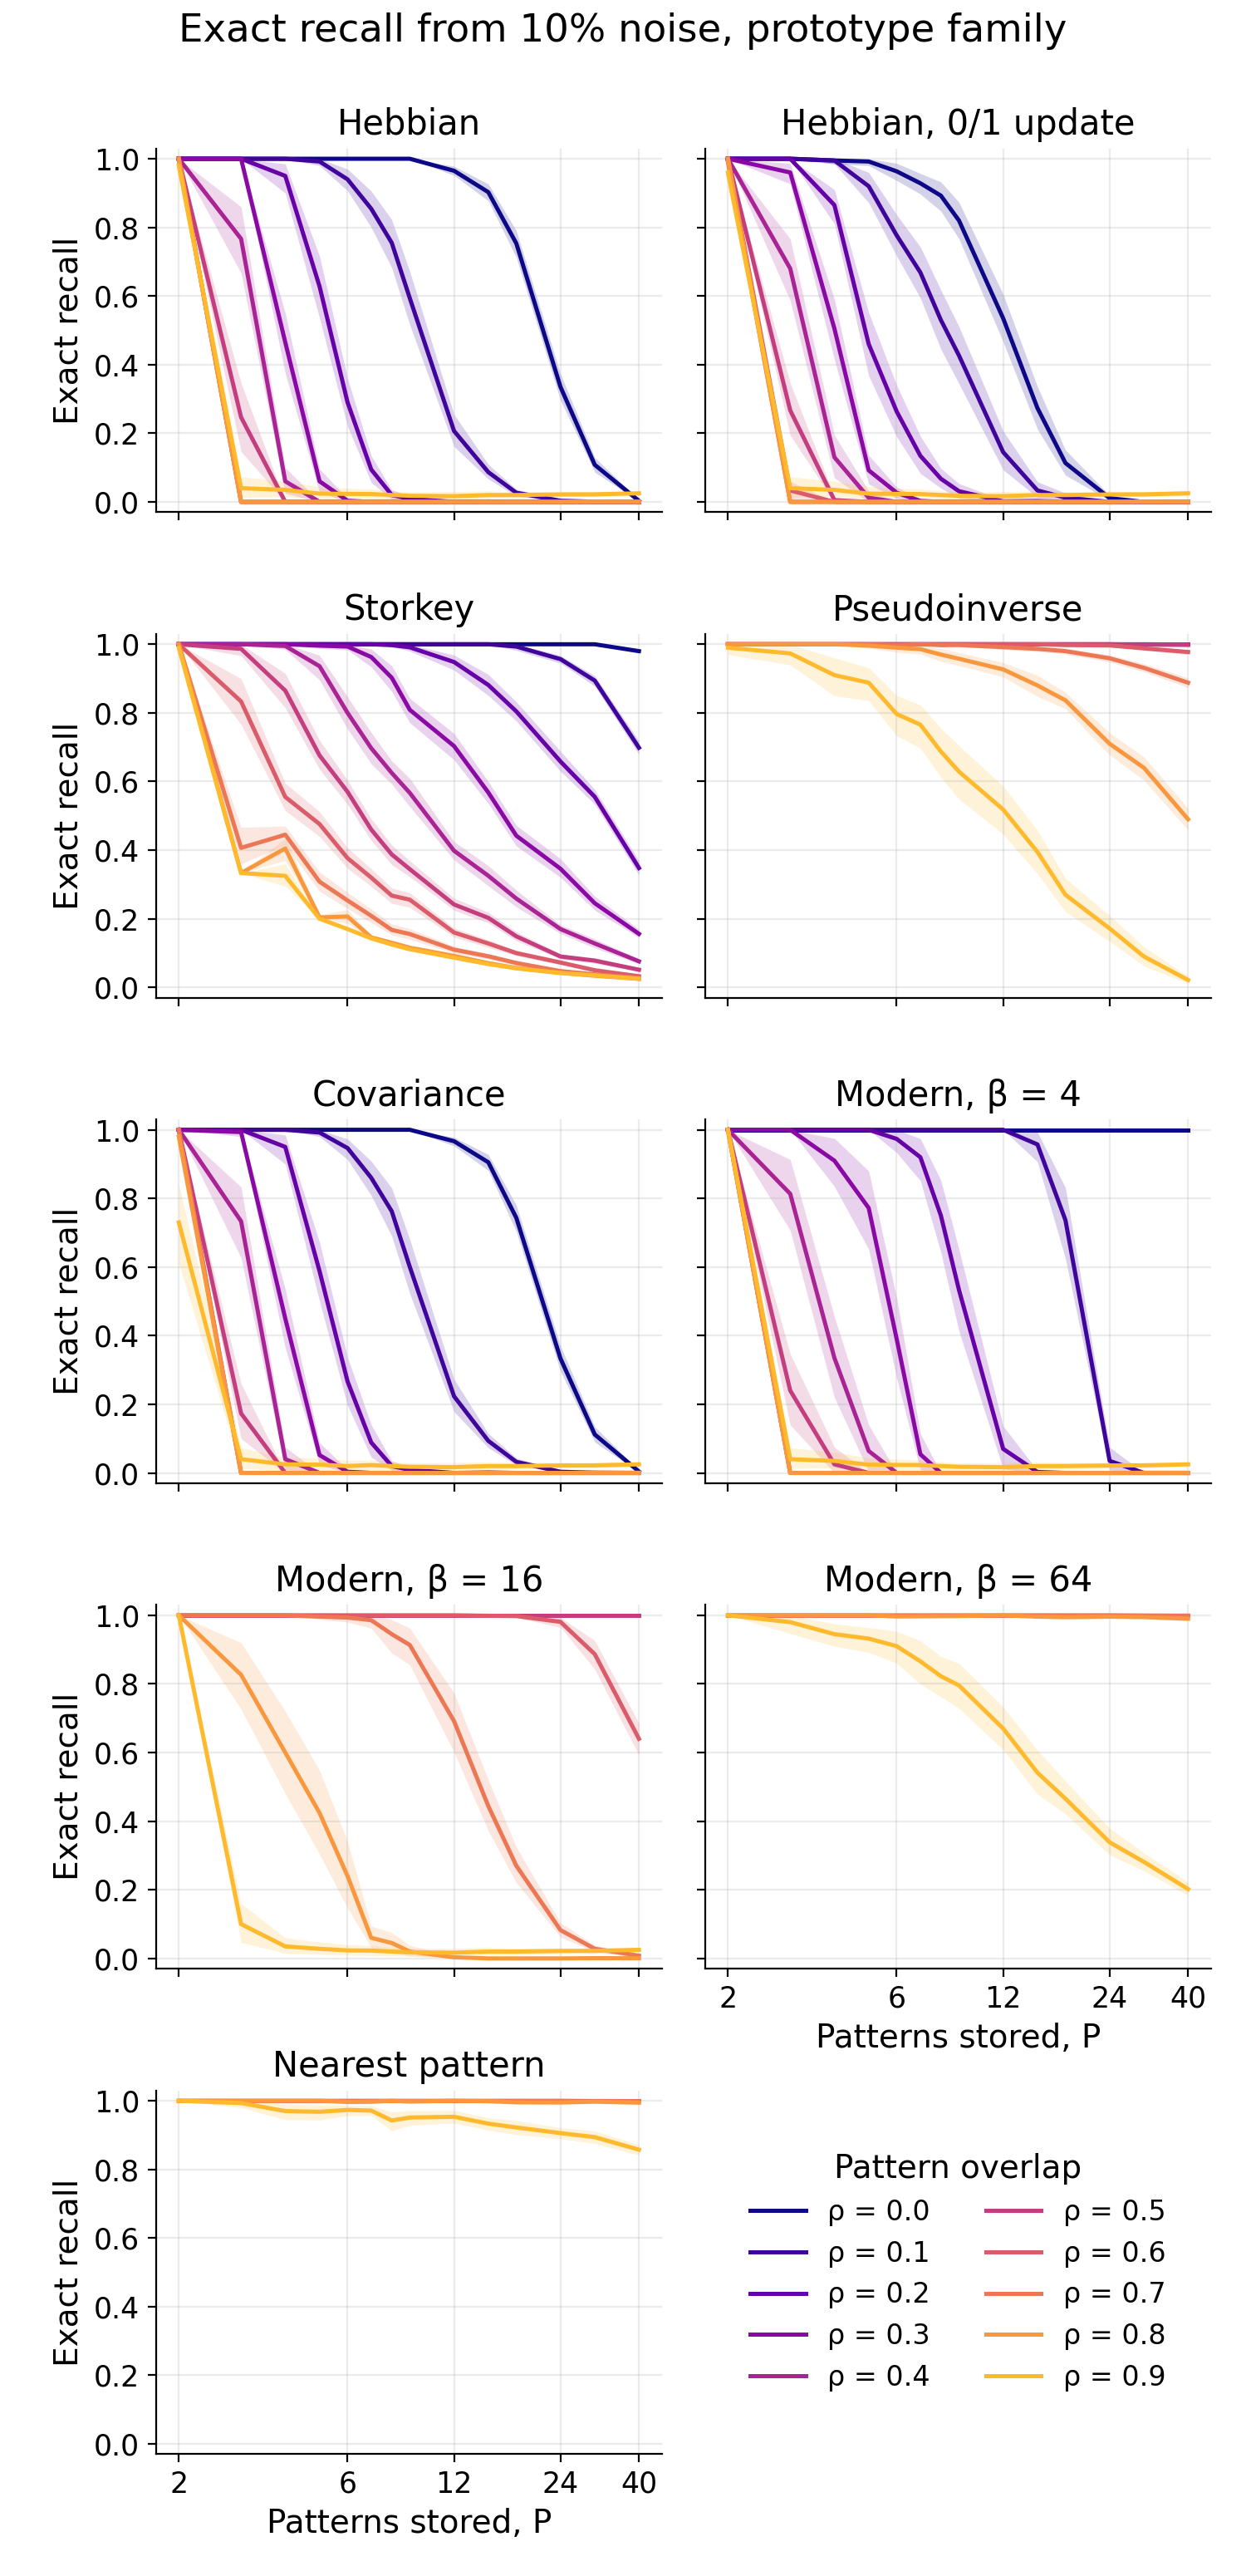
\includegraphics[width=\columnwidth]{../study/figures/fig1_recall_vs_load.png}
\caption{Exact recall from 10\% noise against the number of stored patterns, one panel per rule and one curve per overlap $\rho$, prototype family. Bands are 95\% intervals over 50 pattern sets.}
\label{fig:recall}
\end{figure}

\begin{table*}[t]
\caption{Capacity $P_{50}$ (patterns) at 10\% noise, with 95\% intervals; the modern columns give $\beta$. ``2--3'' means recall fell below 50\% between 2 and 3 stored patterns, and ``$>$40'' means it did not fall below 50\% by 40.}
\label{tab:capacity}
\centering
\scriptsize
\setlength{\tabcolsep}{2pt}
\begin{tabular}{@{}lcccccccc@{}}
\toprule
Condition & Hebbian & Hebb.\ 0/1 & Storkey & Covariance & Pseudoinv. & Modern 16 & Modern 64 & Nearest \\
\midrule
$\rho=0.0$ & 21.4 (21.0--21.9) & 12.4 (11.6--13.1) & $>$40 & 21.4 (20.9--21.8) & $>$40 & $>$40 & $>$40 & $>$40 \\
$\rho=0.1$ & 9.6 (9.1--10.1) & 8.3 (7.6--9.1) & $>$40 & 9.7 (9.2--10.2) & $>$40 & $>$40 & $>$40 & $>$40 \\
$\rho=0.2$ & 5.4 (5.1--5.6) & 4.9 (4.7--5.2) & 32.4 (31.6--33.2) & 5.3 (5.0--5.5) & $>$40 & $>$40 & $>$40 & $>$40 \\
$\rho=0.3$ & 3.9 (3.8--4.1) & 4.0 (3.8--4.2) & 16.6 (15.9--17.2) & 3.9 (3.8--4.1) & $>$40 & $>$40 & $>$40 & $>$40 \\
$\rho=0.4$ & 3.3 (3.2--3.4) & 3.3 (3.2--3.4) & 10.1 (9.5--10.6) & 3.3 (3.2--3.4) & $>$40 & $>$40 & $>$40 & $>$40 \\
$\rho=0.5$ & 2--3 & 2--3 & 6.6 (6.4--6.9) & 2--3 & $>$40 & $>$40 & $>$40 & $>$40 \\
$\rho=0.6$ & 2--3 & 2--3 & 4.7 (4.3--5.1) & 2--3 & $>$40 & $>$40 & $>$40 & $>$40 \\
$\rho=0.7$ & 2--3 & 2--3 & 2--3 & 2--3 & $>$40 & 14.3 (13.3--15.3) & $>$40 & $>$40 \\
$\rho=0.8$ & 2--3 & 2--3 & 2--3 & 2--3 & 39.2 (37.0--$>$40) & 4.5 (3.9--5.2) & $>$40 & $>$40 \\
$\rho=0.9$ & 2--3 & 2--3 & 2--3 & 2--3 & 12.4 (10.4--13.8) & 2--3 & 16.6 (14.5--18.6) & $>$40 \\
\midrule
density 0.65 & 10.7 (10.2--11.2) & 3.8 (3.7--4.0) & $>$40 & 23.8 (23.2--24.4) & $>$40 & $>$40 & $>$40 & $>$40 \\
density 0.80 & 3.5 (3.5--3.6) & 2--3 & 11.8 (11.2--12.7) & 29.2 (28.6--30.0) & $>$40 & $>$40 & $>$40 & $>$40 \\
\bottomrule
\end{tabular}

\end{table*}

By capacity, the rules keep a stable order on prototype patterns, at both noise levels, wherever their capacities can be told apart. Hebbian and covariance sit lowest on shared structure, Storkey above them, the pseudoinverse rule above that, and the modern network at $\beta = 64$ and nearest-pattern lookup on top. At 10\% noise, Storkey keeps $P_{50}$ above 40 up to $\rho = 0.1$ (\N{c:proto:0.1:storkey:20} at 20\% noise) and degrades smoothly: \N{c:proto:0.2:storkey:10} at $\rho = 0.2$, \N{c:proto:0.4:storkey:10} at 0.4, and \N{c:proto:0.5:storkey:10} at 0.5. From $\rho = 0.7$, its crossing also lies between 2 and 3 patterns, but at three patterns, it still recalls \N{r:proto:0.7:storkey:10:3} at $\rho = 0.7$ and \N{r:proto:0.8:storkey:10:3} at 0.8 and 0.9, where Hebbian recalls \N{r:proto:0.7:hebb:10:3} to \N{r:proto:0.9:hebb:10:3}. At 10\% noise, the pseudoinverse rule holds $P_{50}$ above 40 up to $\rho = 0.7$ (\N{c:proto:0.8:pinv:10} at 0.8, \N{c:proto:0.9:pinv:10} at 0.9), and at 20\% noise, up to $\rho = 0.6$ (\N{c:proto:0.7:pinv:20} at 0.7). The modern network at $\beta = 64$ holds to $\rho = 0.8$ and reaches \N{c:proto:0.9:modern64:10} at 0.9; at $\beta = 16$, it reaches \N{c:proto:0.7:modern16:10} at 0.7 and \N{c:proto:0.8:modern16:10} at 0.8. At $\beta = 4$, the modern network falls below Storkey from $\rho = 0.1$ to 0.6 (Fig.~\ref{fig:recall}): at 10\% noise, \N{c:proto:0.1:modern4:10} at $\rho = 0.1$ and \N{c:proto:0.4:modern4:10} at 0.4, against Storkey's above 40 and \N{c:proto:0.4:storkey:10}.

\begin{figure}[t]
\centering
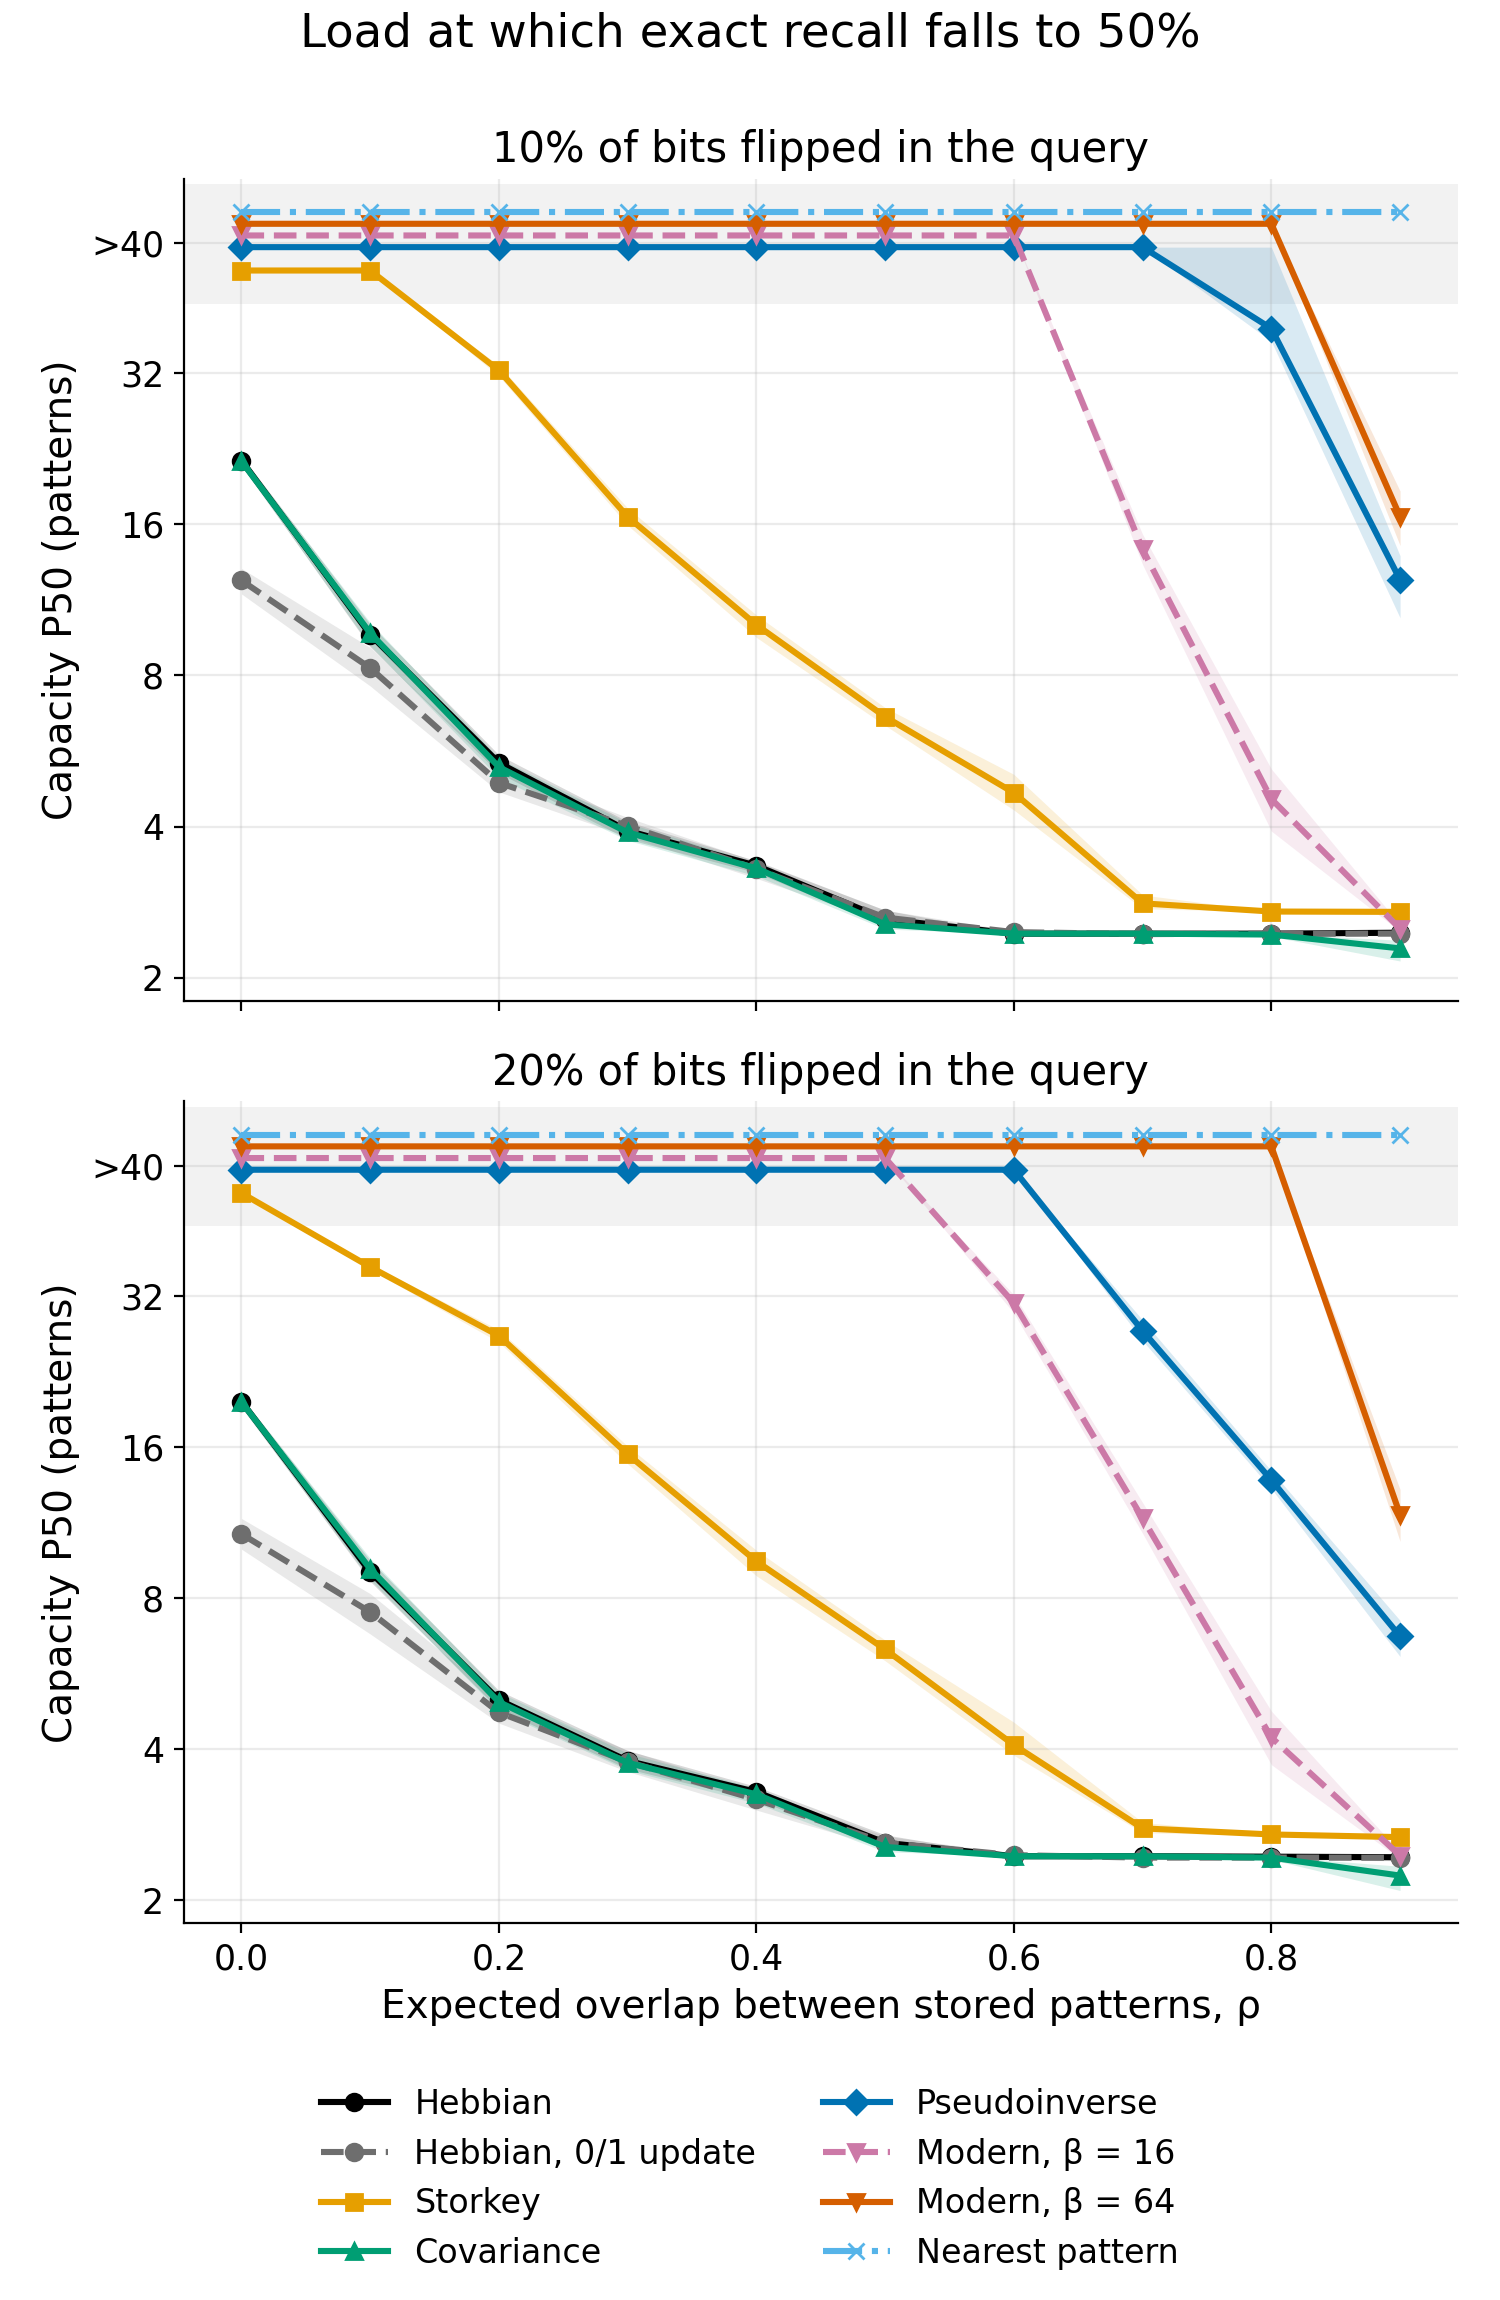
\includegraphics[width=\columnwidth]{../study/figures/fig2_capacity_vs_overlap.png}
\caption{Capacity $P_{50}$ against expected overlap $\rho$, prototype family, at 10\% and 20\% noise. The log axis runs from 2 to 40 patterns. Capacities above 40 are drawn in the shaded band at the top, offset by rule so the lines stay apart, so a value just under 40, such as the pseudoinverse rule's \N{c:proto:0.8:pinv:10} at $\rho = 0.8$, sits below the band. Values between 2 and 3 are interpolated between the two loads tested there; small capacities are compared through recall at $P = 3$.}
\label{fig:capacity}
\end{figure}

\subsection{The assignment's update costs capacity}

The assignment's 0/1 update is the standard update plus the bias in~\eqref{eq:bias}. On independent balanced patterns, it lowers the Hebbian $P_{50}$ from \N{c:proto:0.0:hebb:10} to \N{c:proto:0.0:hebb01:10} [\N{c:proto:0.0:hebb01:10:lo}, \N{c:proto:0.0:hebb01:10:hi}], a loss of \N{g:hebb01_loss_pct}\% at 10\% noise (\N{c:proto:0.0:hebb:20} to \N{c:proto:0.0:hebb01:20} at 20\%). At 18 stored patterns, the standard update recalls \N{r:proto:0.0:hebb:10:18} of them and the 0/1 update \N{r:proto:0.0:hebb01:10:18} (10\% noise); at 20\% noise, the figures are \N{r:proto:0.0:hebb:20:18} and \N{r:proto:0.0:hebb01:20:18}. Figure~\ref{fig:update} shows the curves.

\begin{figure}[t]
\centering
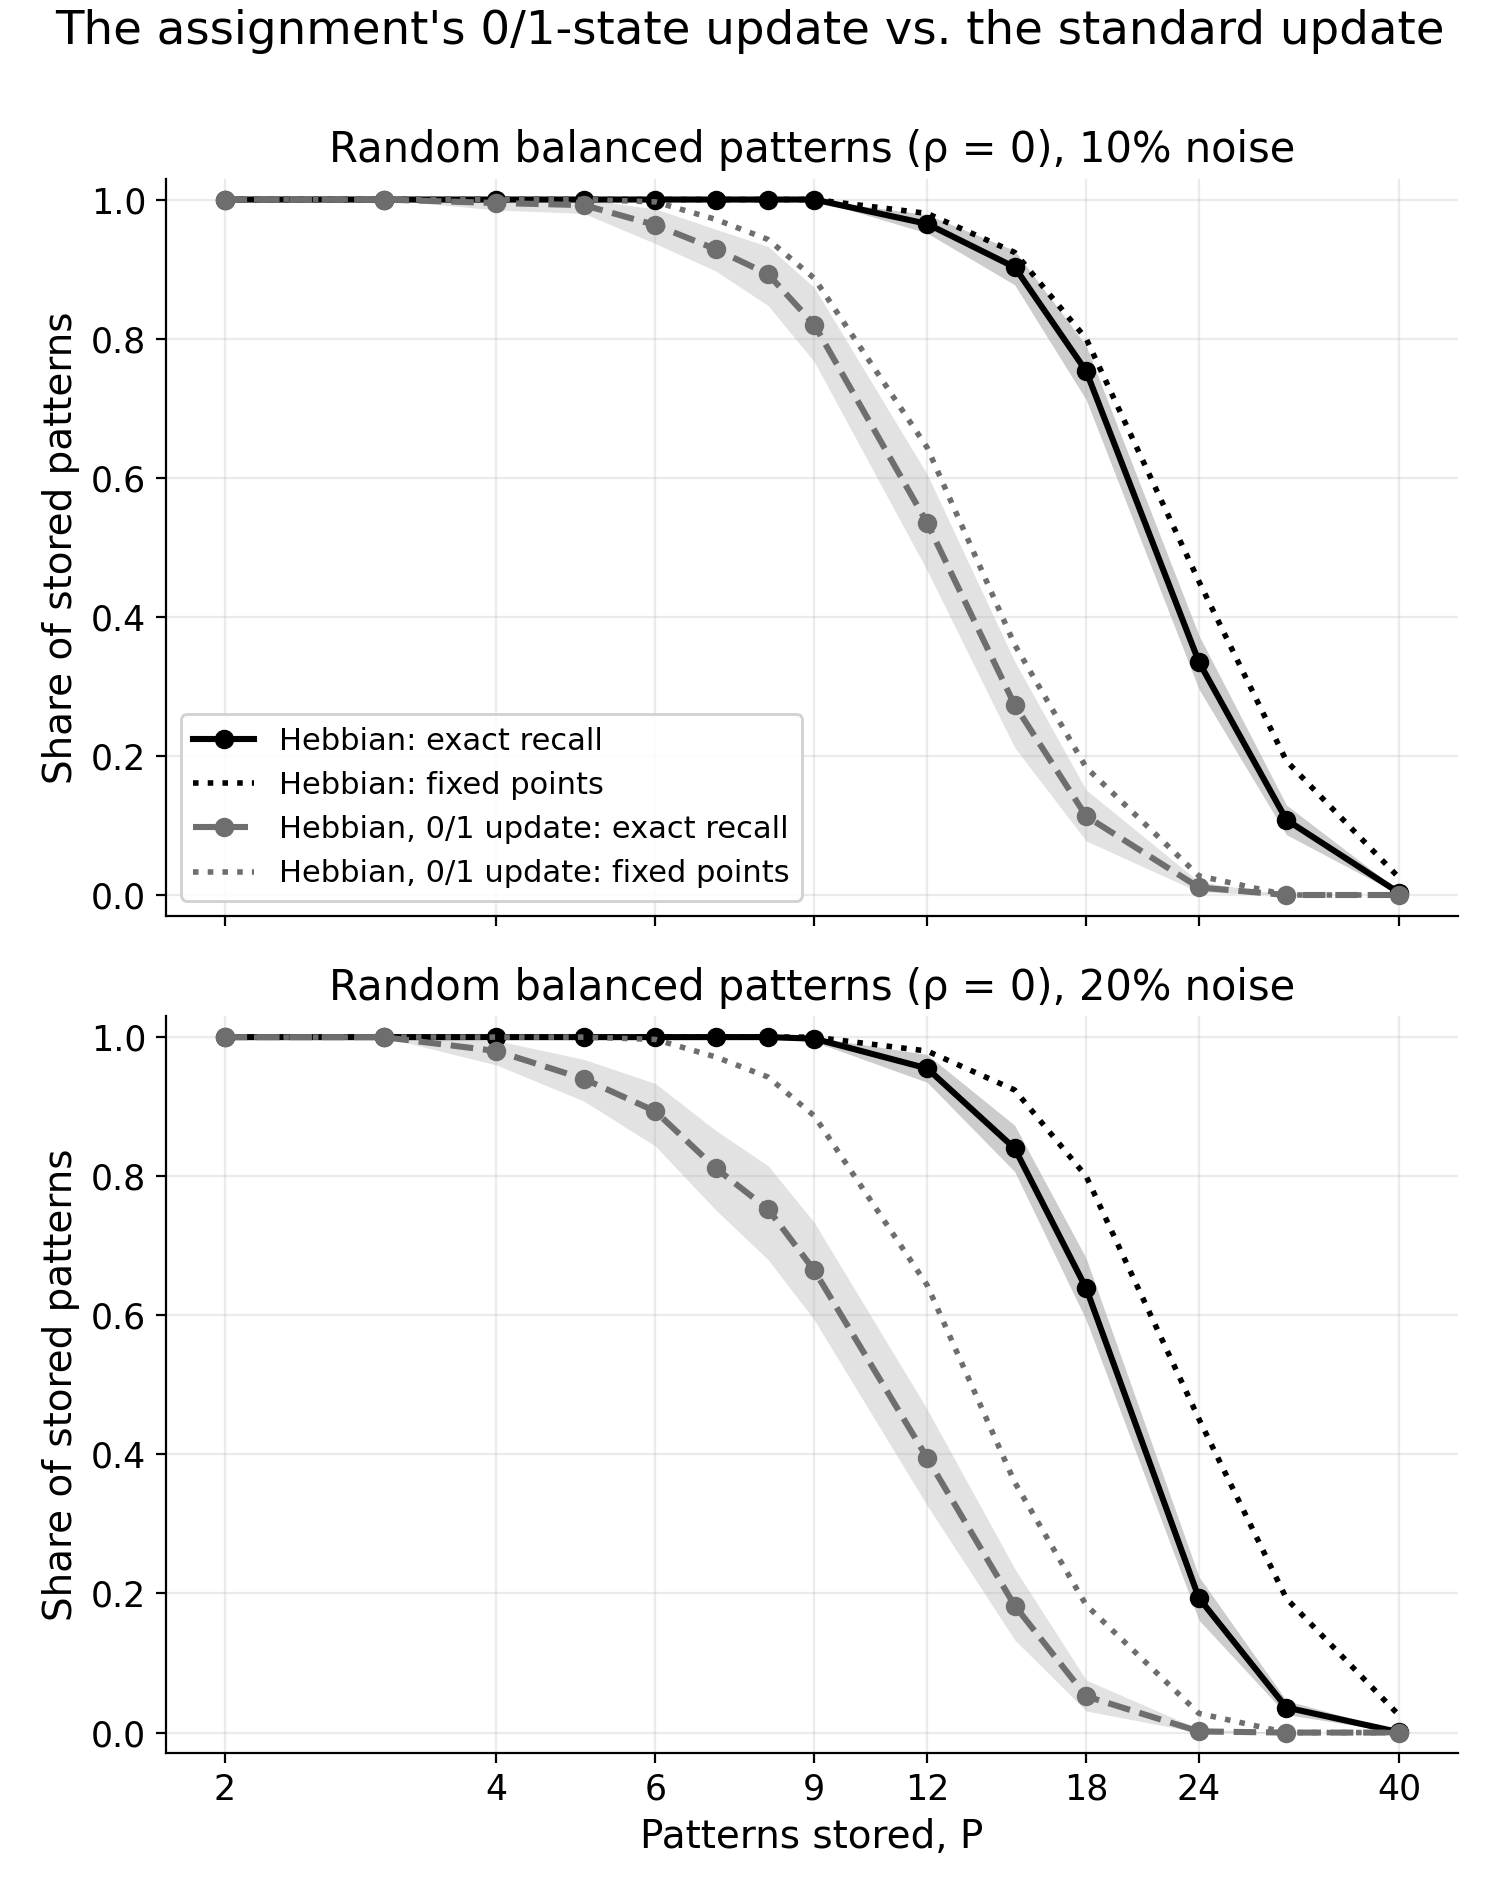
\includegraphics[width=\columnwidth]{../study/figures/fig6_assignment_update.png}
\caption{Hebbian weights under the assignment's 0/1 update (dashed) and the standard $\pm 1$ update (solid), for independent balanced patterns ($\rho = 0$) at 10\% (top) and 20\% (bottom) noise. Lines with markers are exact recall, with 95\% bands over 50 pattern sets; dotted lines are the share of stored patterns that are fixed points.}
\label{fig:update}
\end{figure}

\subsection{Density and shared structure}

Two conditions have a similar mean overlap. Independent bits at density 0.80 have an overlap of \N{po:biased:0.8}, and the prototype family at $\rho = 0.4$ has \N{po:proto:0.4}. Both break Hebbian storage: $P_{50}$ is \N{c:biased:0.8:hebb:10} and \N{c:proto:0.4:hebb:10}, and recall at 18 patterns is \N{r:biased:0.8:hebb:10:18} in both. The covariance rule, which removes the density effect, separates them (Fig.~\ref{fig:density}). It reaches \N{c:biased:0.8:cov:10} [\N{c:biased:0.8:cov:10:lo}, \N{c:biased:0.8:cov:10:hi}] on the biased patterns, with recall \N{r:biased:0.8:cov:10:18} at 18 patterns, but only \N{c:proto:0.4:cov:10} [\N{c:proto:0.4:cov:10:lo}, \N{c:proto:0.4:cov:10:hi}] on the prototype patterns. Storkey's capacities on the two are close (\N{c:biased:0.8:storkey:10} and \N{c:proto:0.4:storkey:10}), unlike the covariance rule's. At independent bits with density 0.65, where the overlap is small (\N{po:biased:0.65:4}), Hebbian $P_{50}$ is \N{c:biased:0.65:hebb:10}. This compares two specific conditions and is not a controlled decomposition. The covariance rule's \N{c:biased:0.8:cov:10} exceeds Hebbian's \N{c:proto:0.0:hebb:10} on balanced patterns, likely because biased patterns carry less information each, which would make it a different regime and not a return to the balanced level; the study does not test this.

At $\rho = 0$, the covariance rule matches Hebbian: their recall differs by at most \N{v:max_abs_diff} at every load and noise level, paired by pattern set. Of the \N{v:n_total} paired intervals, \N{v:n_zero} are $[0, 0]$ because the two rules score the same on every pattern set, so they test nothing; of the other \N{v:n_informative}, \N{v:n_excl_zero} excludes zero (load \N{v:excl_P} at \N{v:excl_noise}\% noise, difference \N{v:excl_diff}, interval [\N{v:excl_lo}, \N{v:excl_hi}]).

\begin{figure}[t]
\centering
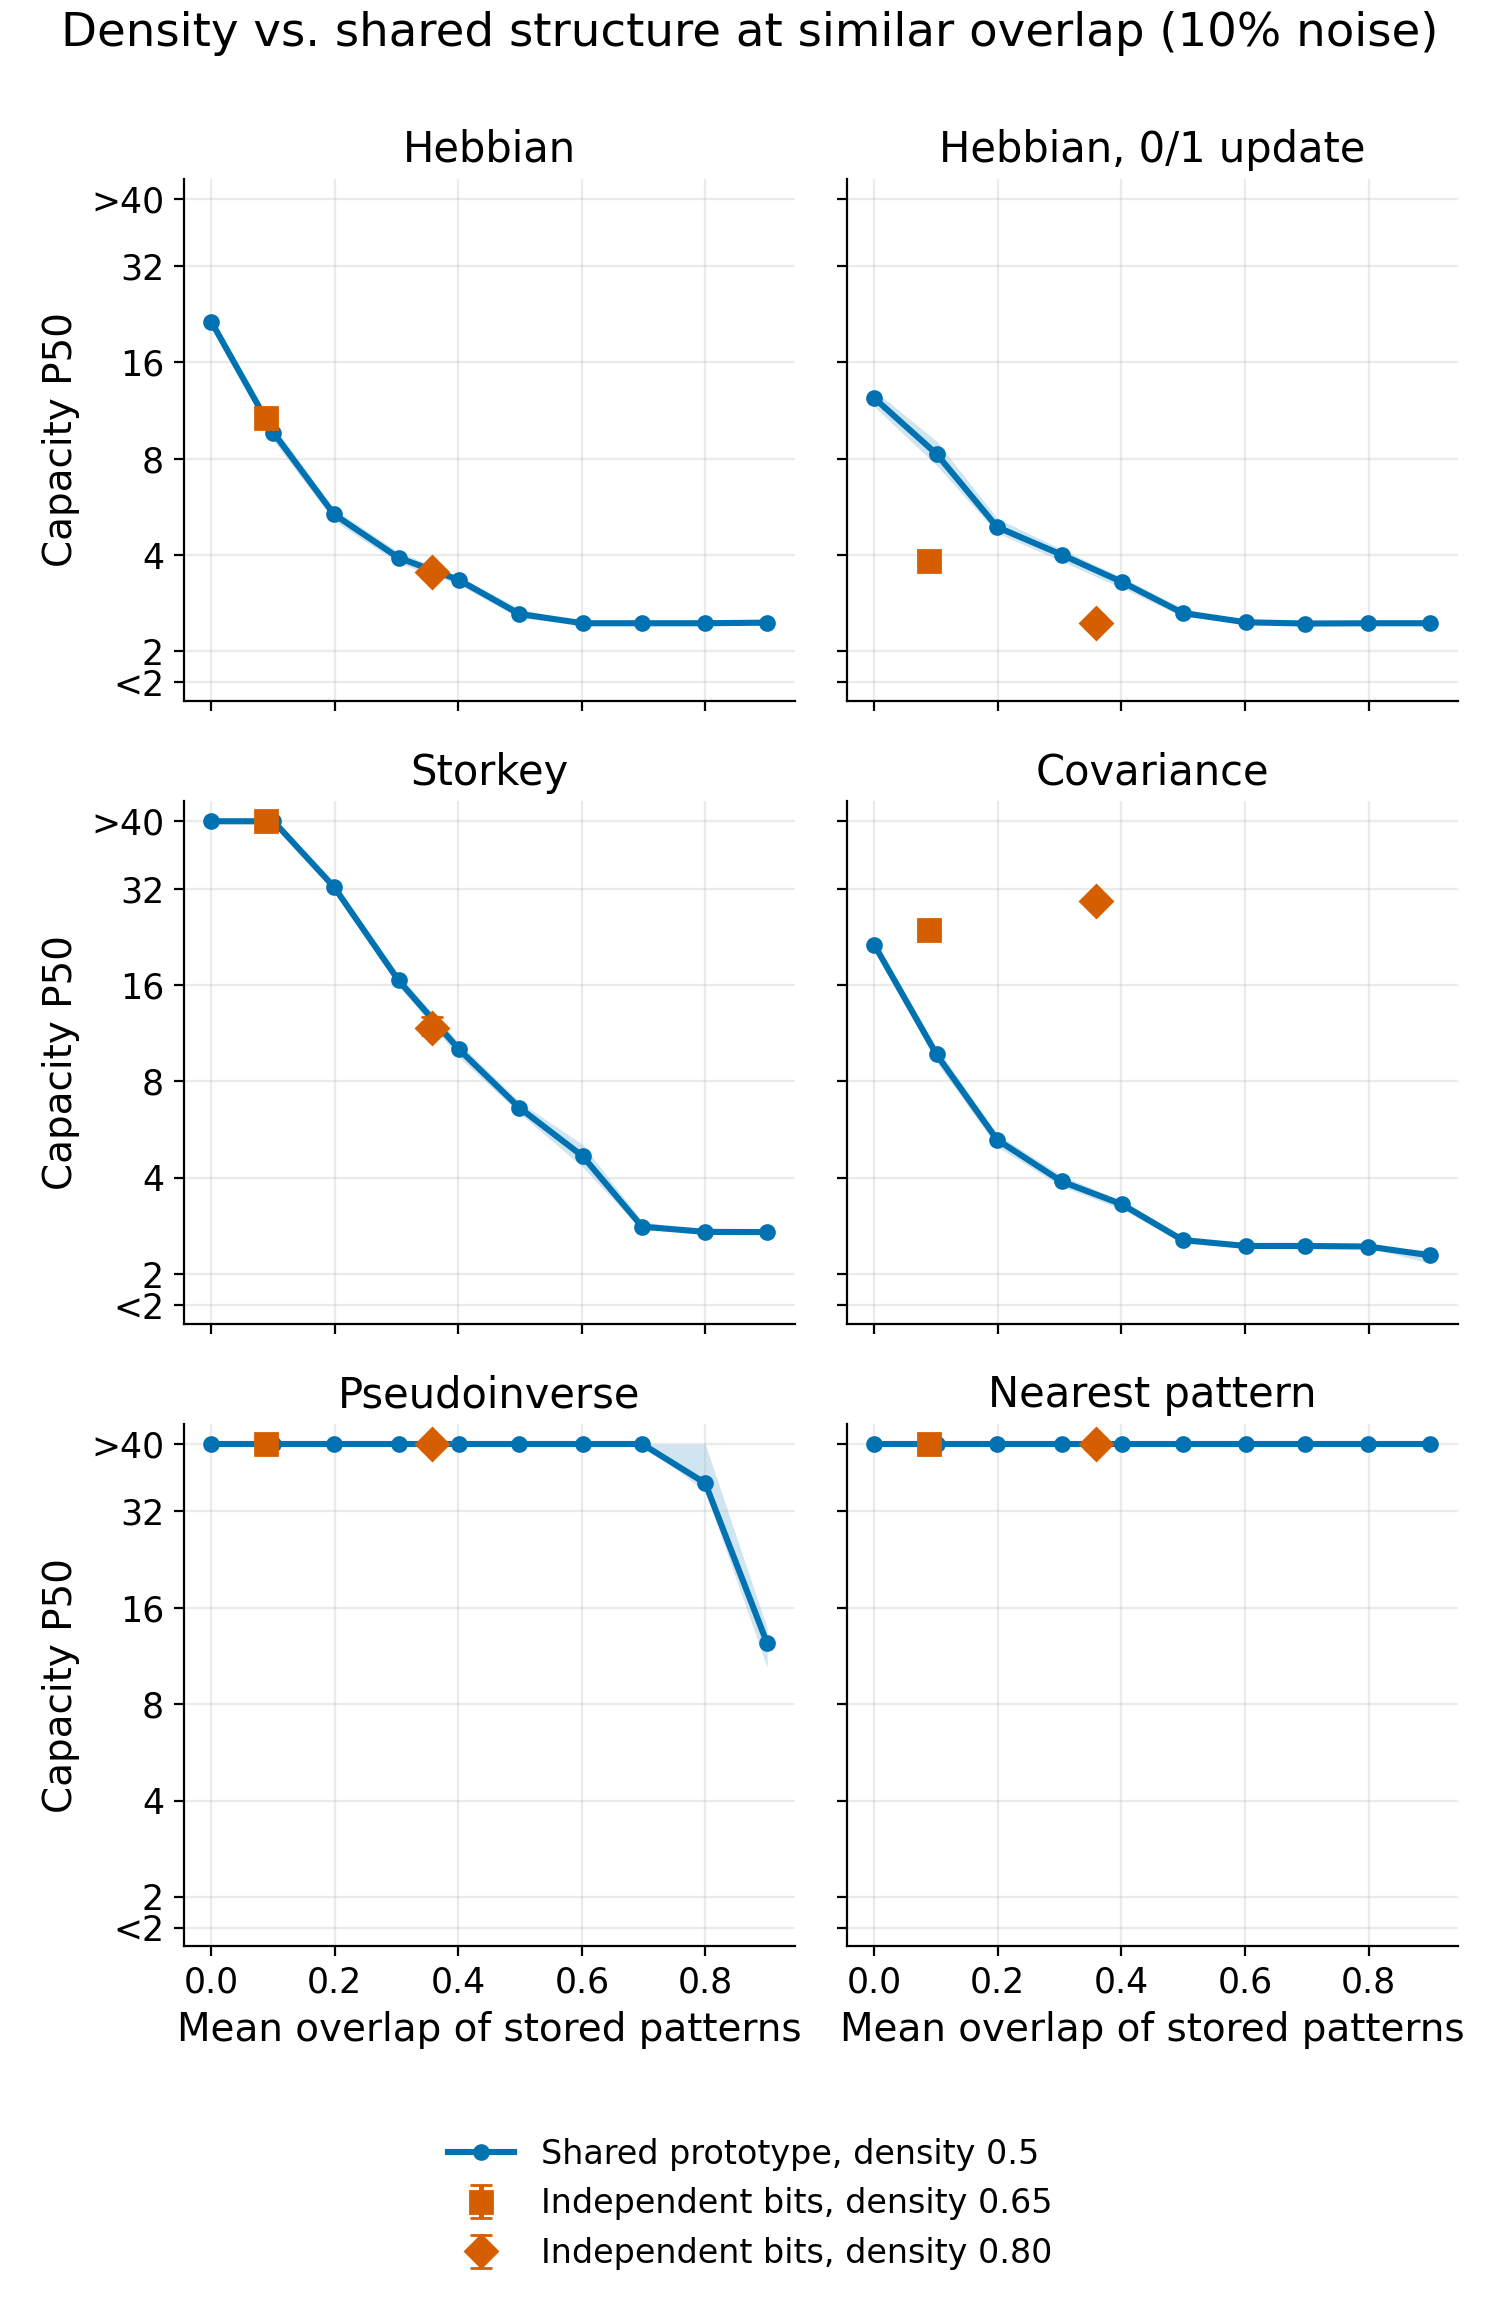
\includegraphics[width=\columnwidth]{../study/figures/fig3_density_vs_structure.png}
\caption{Capacity at 10\% noise for the prototype family (line) and for independent biased bits (squares: density 0.65; diamonds: density 0.80), against mean pattern overlap. Values between 2 and 3 are interpolated between the two loads tested there; small capacities are compared through recall at $P = 3$.}
\label{fig:density}
\end{figure}
